\documentclass[crop,tikz]{standalone}

\usepackage{amsmath}

\usetikzlibrary{arrows}
\usetikzlibrary{positioning}

\begin{document}
  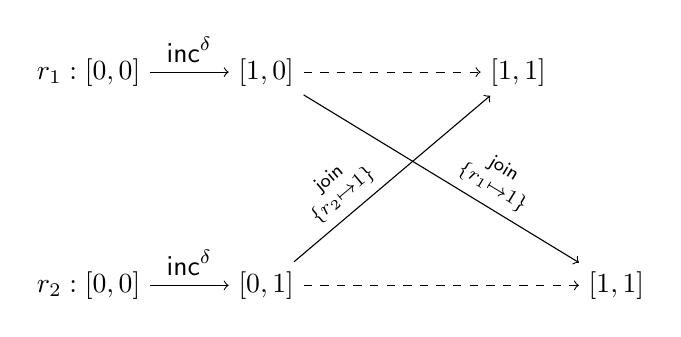
\begin{tikzpicture}
    \node (r1a) {$r_1:[0,0]$};
    \node (r2a) [below = 6em of r1a] {$r_2:[0,0]$};

    \node (r1b) [right = of r1a] {$[1,0]$};
    \node (r2b) [right = of r2a] {$[0,1$]};

    \node (r1c) [right = of r1b] {};
    \node (r2e) [right = of r2b] {};
    \node (r2c) [right = of r2e] {};

    \node (r1d) [right = of r1c] {$[1,1]$};
    \node (r2d) [right = of r2c] {$[1,1]$};

    \draw [->] (r1a) -- node [above] {$\textsf{inc}^\delta$} (r1b);
    \draw [->] (r2a) -- node [above] {$\textsf{inc}^\delta$} (r2b);

    \draw [->,dashed] (r1b) -- (r1d);
    \draw [->] (r2b) -- node [midway, sloped, above left] {$\substack{\textsf{join}\\\{r_2 \mapsto 1\}}$} (r1d);

    \draw [->,dashed] (r2b) -- (r2d);
    \draw [->] (r1b) -- node [midway, sloped, above right] {$\substack{\textsf{join}\\\{r_1 \mapsto 1\}}$} (r2d);
  \end{tikzpicture}
\end{document}
